\documentclass[]{book}
\usepackage{lmodern}
\usepackage{amssymb,amsmath}
\usepackage{ifxetex,ifluatex}
\usepackage{fixltx2e} % provides \textsubscript
\ifnum 0\ifxetex 1\fi\ifluatex 1\fi=0 % if pdftex
  \usepackage[T1]{fontenc}
  \usepackage[utf8]{inputenc}
\else % if luatex or xelatex
  \ifxetex
    \usepackage{mathspec}
  \else
    \usepackage{fontspec}
  \fi
  \defaultfontfeatures{Ligatures=TeX,Scale=MatchLowercase}
\fi
% use upquote if available, for straight quotes in verbatim environments
\IfFileExists{upquote.sty}{\usepackage{upquote}}{}
% use microtype if available
\IfFileExists{microtype.sty}{%
\usepackage{microtype}
\UseMicrotypeSet[protrusion]{basicmath} % disable protrusion for tt fonts
}{}
\usepackage[margin=1in]{geometry}
\usepackage{hyperref}
\hypersetup{unicode=true,
            pdftitle={Badania Internetowe},
            pdfauthor={Maciej Beręsewicz},
            pdfborder={0 0 0},
            breaklinks=true}
\urlstyle{same}  % don't use monospace font for urls
\usepackage{natbib}
\bibliographystyle{apalike}
\usepackage{longtable,booktabs}
\usepackage{graphicx,grffile}
\makeatletter
\def\maxwidth{\ifdim\Gin@nat@width>\linewidth\linewidth\else\Gin@nat@width\fi}
\def\maxheight{\ifdim\Gin@nat@height>\textheight\textheight\else\Gin@nat@height\fi}
\makeatother
% Scale images if necessary, so that they will not overflow the page
% margins by default, and it is still possible to overwrite the defaults
% using explicit options in \includegraphics[width, height, ...]{}
\setkeys{Gin}{width=\maxwidth,height=\maxheight,keepaspectratio}
\IfFileExists{parskip.sty}{%
\usepackage{parskip}
}{% else
\setlength{\parindent}{0pt}
\setlength{\parskip}{6pt plus 2pt minus 1pt}
}
\setlength{\emergencystretch}{3em}  % prevent overfull lines
\providecommand{\tightlist}{%
  \setlength{\itemsep}{0pt}\setlength{\parskip}{0pt}}
\setcounter{secnumdepth}{5}
% Redefines (sub)paragraphs to behave more like sections
\ifx\paragraph\undefined\else
\let\oldparagraph\paragraph
\renewcommand{\paragraph}[1]{\oldparagraph{#1}\mbox{}}
\fi
\ifx\subparagraph\undefined\else
\let\oldsubparagraph\subparagraph
\renewcommand{\subparagraph}[1]{\oldsubparagraph{#1}\mbox{}}
\fi

%%% Use protect on footnotes to avoid problems with footnotes in titles
\let\rmarkdownfootnote\footnote%
\def\footnote{\protect\rmarkdownfootnote}

%%% Change title format to be more compact
\usepackage{titling}

% Create subtitle command for use in maketitle
\newcommand{\subtitle}[1]{
  \posttitle{
    \begin{center}\large#1\end{center}
    }
}

\setlength{\droptitle}{-2em}
  \title{Badania Internetowe}
  \pretitle{\vspace{\droptitle}\centering\huge}
  \posttitle{\par}
  \author{Maciej Beręsewicz}
  \preauthor{\centering\large\emph}
  \postauthor{\par}
  \predate{\centering\large\emph}
  \postdate{\par}
  \date{2016-12-28}

\usepackage{booktabs}

\begin{document}
\maketitle

{
\setcounter{tocdepth}{1}
\tableofcontents
}
\chapter{Badania internetowe -- podstawowe
wymagania}\label{badania-internetowe-podstawowe-wymagania}

\chapter{Wprowadzenie do badań internetowych}\label{intro}

\chapter{Konstrukcja i przykłady
badań}\label{konstrukcja-i-przykady-badan}

\chapter{Technologie w badaniach
internetowych}\label{technologie-w-badaniach-internetowych}

\chapter{Paradane}\label{paradane}

\section{Paradane -- definicja}\label{paradane-definicja}

Definicje za \citep{kreuter2013improving}

\textbf{Paradata} are data generated in the process of conducting a
survey; generated as a by-product of computer-assisted data collection.

Respondents in web surveys leave electronic traces as they answer survey
questions, captured through their keystrokes and mouse clicks. In
telephone surveys, automated call scheduling systems record the date and
time of every call. In face-to-face surveys, interviewers' keystrokes
are easily captured alongside the interview and so are audio or even
video recordings of the respondent-- interviewer interactions. Each of
these is an example of paradata available through the computerized
survey software.

Paradata vs Metadata.

Paradata vs Zmienne Pomocniczne (ang. auxiliary variables).

\section{Znaczenie paradanych}\label{znaczenie-paradanych}

\begin{figure}[htbp]
\centering
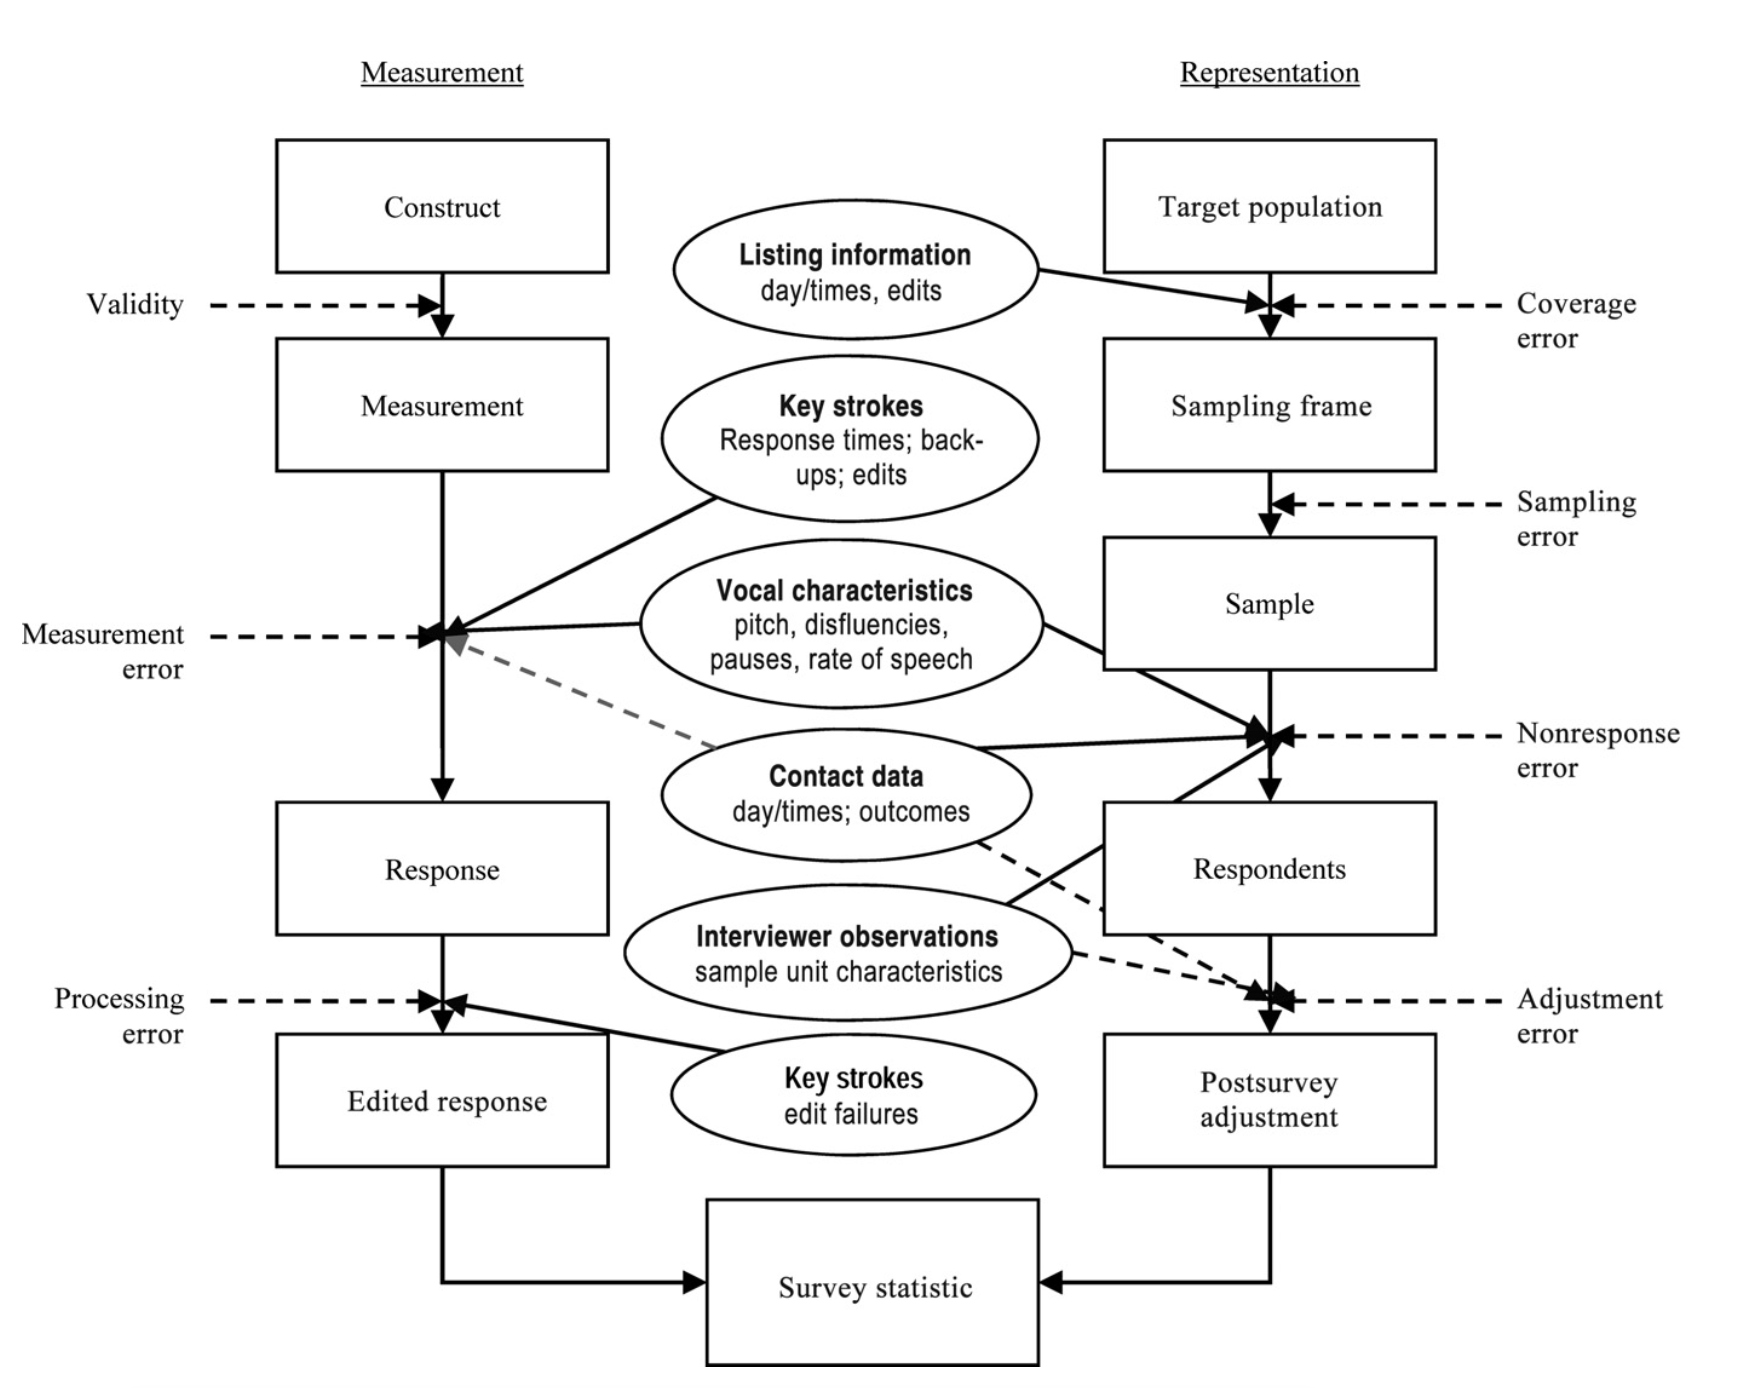
\includegraphics{imgs/paradata-tse.png}
\caption{Znaczenie paradanych. Źródło:
\citet{kreuter2013improving},Rozdział 1}
\end{figure}

\section{Przykłady wykorzystania}\label{przykady-wykorzystania}

\section{Dalsze kroki}\label{dalsze-kroki}

\chapter{Dobór próby w badaniach
internetowych}\label{dobor-proby-w-badaniach-internetowych}

\chapter{Jakość badań internetowych}\label{jakosc-badan-internetowych}

\chapter{Ważenie danych}\label{wazenie-danych}

\chapter{Estymacja w badaniach
internetowych}\label{estymacja-w-badaniach-internetowych}

\chapter{Big data i inne nowe źródła
danych}\label{big-data-i-inne-nowe-zroda-danych}

\chapter{Wybrane problemy}\label{wybrane-problemy}

\chapter{Placeholder}\label{placeholder}

\bibliography{packages.bib,book.bib}


\end{document}
